
\tikzstyle{block} = [rectangle, draw, fill=blue!20,text centered, rounded corners, minimum height=3em, node distance=2cm]
\tikzstyle{cloud} = [ellipse,   draw, fill=red!20, text badly centered, node distance=2cm]

\begin{frame}<1>[label=mctstructure]{mctracer Struktur}
	%\begin{block}
		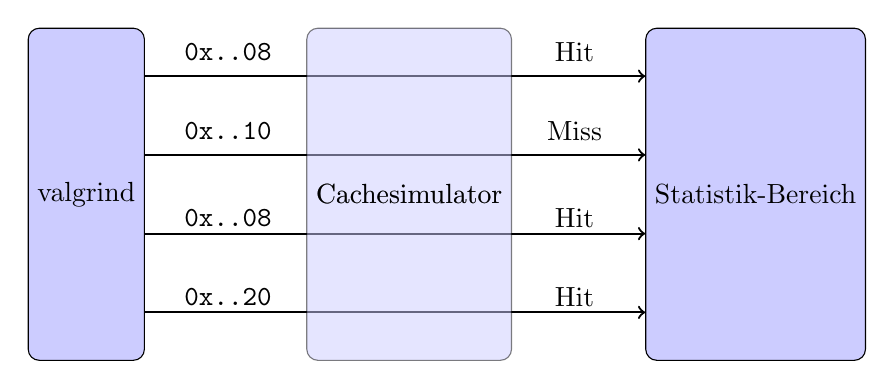
\begin{tikzpicture}
			\node [block,minimum height=120] (valg) at (0,0) {valgrind};
			\node [block,minimum height=120] (stat) at (8.5,0) {Statistik-Bereich};
			\path [draw,->,thick] ([yshift=1.5cm]valg.east) -- ([yshift=1.5cm]stat.west);
			\path [draw,->,thick] ([yshift=0.5cm]valg.east) -- ([yshift=0.5cm]stat.west);
			\path [draw,->,thick] ([yshift=-0.5cm]valg.east) -- ([yshift=-0.5cm]stat.west);
			\path [draw,->,thick] ([yshift=-1.5cm]valg.east) -- ([yshift=-1.5cm]stat.west);
			\node [block,minimum height=120,opacity=0.5] (csim) at (4.1,0) {Cachesimulator};
			\node at (4.1,0) {Cachesimulator};
			\node at (1.8,-1.3cm) {\texttt{0x..20}};
			\node at (1.8,-0.3cm) {\texttt{0x..08}};
			\node at (1.8,0.8cm) {\texttt{0x..10}};
			\node at (1.8,1.8cm) {\texttt{0x..08}};
			\node at (6.2,-1.3cm) {Hit};
			\node at (6.2,-0.3cm) {Hit};
			\node at (6.2,0.8cm) {Miss};
			\node at (6.2,1.8cm) {Hit};
		\end{tikzpicture}
	%\end{block}
\end{frame}

\begin{frame}{Cachesimulator}
	\begin{block}{Cachesimulator}
		\begin{itemize}[<+->]
			\item mengenassoziativ
			\item Realisiert über ein Array aus Tags
			\item Tag gibt zu einer Cachezelle die gecachteSpeicheradresse an
			\item Mehrere nebeneinanderliegende Tags werden zu einem Set zusammengefasst
			\item Bei einem Speicherzugriff wird die Speicheradresse in ein Set abgebildet
			\item Alle Tags dieses Sets werden überprüft, bei einer Übereinstimmung handelt es sich um einen Hit
			\item Bei einem miss wird der Tag des Zugriffs an den anfang des Sets geschrieben und alle anderen nach hinten verdrängt
		\end{itemize}
	\end{block}
\end{frame}

\againframe<2>{mctstructure}

\begin{frame}{Statistik-Bereich}
	\begin{tikzpicture}
		\node [cloud] (accev) {Speicherzugriffe};
		\onslide<2->{
			\node [block, below of=accev] (calc) {Reverse Adressrechnung};
			\path [draw,->] (accev) -- (calc);
			\node [cloud] (absstat) at (5.7,-1.7) {Zugriffe pro Matrix-Zelle};
			\node [cloud] (relstat) at (5.7,-2.6) {Statistik: Relative Zugriffe};
			\path [draw,->] (calc) -- (absstat.west);
			\path [draw,->] (calc) -- (relstat.west);
		}
		\onslide<3->{
			\node [cloud, below of=calc] (raccv) {Relative Zugriffe};
			\path [draw] (calc) -- (raccv);
			\node [block, below of=raccv] (patseq) {Pattern/Sequence-Logik};
			\path [draw,->] (raccv) -- (patseq);
			\node [cloud] (pat) at (5.7,-5.0) {Muster};
			\node [cloud] (seq) at (5.7,-5.9) {Sequenzen von Mustern};
			\path [draw,->] (patseq.north east) -- (pat.west);
			\path [draw,->] (patseq) -- (seq.west);
		}
	\end{tikzpicture}
\end{frame}

\tikzstyle{accarrw} = [draw,->,thick, shorten <=10, shorten >=10]
\begin{frame}{Patterns, Sequences}
	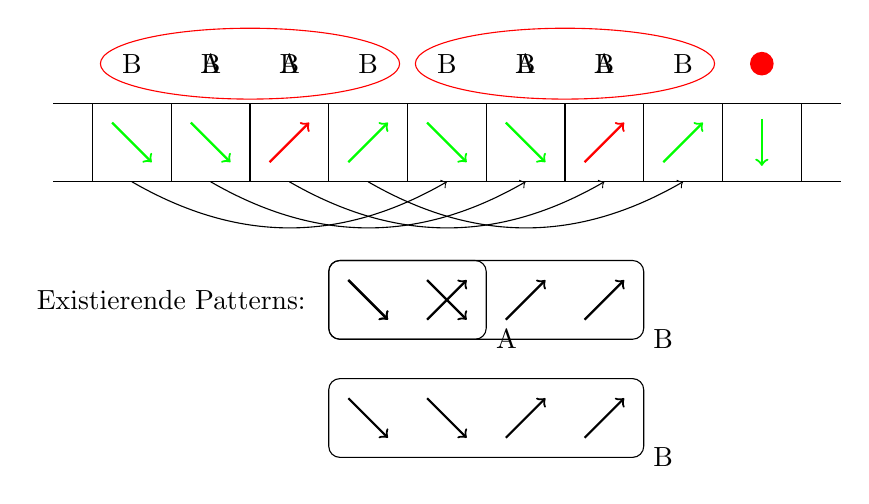
\begin{tikzpicture}
		\draw (-0.5,0) grid (9.5,1);
		\path [accarrw,green] (0,1) -- (1,0);
		\path [accarrw,green] (1,1) -- (2,0);
		\path [accarrw,red]   (2,0) -- (3,1);
		\path [accarrw,green] (3,0) -- (4,1);
		\path [accarrw,green] (4,1) -- (5,0);
		\path [accarrw,green] (5,1) -- (6,0);
		\path [accarrw,red]   (6,0) -- (7,1);
		\path [accarrw,green] (7,0) -- (8,1);
		\path [accarrw,green] (8.5,1.15) -- (8.5,-0.15);
		\node at (1,-1.5) {Existierende Patterns:};
		\onslide<1-5>{
			\path [accarrw] (3,-1) -- (4,-2);
			\path [accarrw] (4,-2) -- (5,-1);
			\draw [rounded corners,] (3,-1) rectangle (5,-2) node [right] {A};
		}
		\onslide<2-5>{
			\node at (1.5,1.5) {A};
			\node at (2.5,1.5) {A};
			\node at (5.5,1.5) {A};
			\node at (6.5,1.5) {A};
		}
		\onslide<3-4>{
			\draw [->] (0.5,0) to [bend right](4.5,0);
		}
		\onslide<4>{
			\draw [->] (1.5,0) to [bend right](5.5,0);
			\draw [->] (2.5,0) to [bend right](6.5,0);
			\draw [->] (3.5,0) to [bend right](7.5,0);
		}
		\onslide<5>{
			\path [accarrw] (3,-2.5) -- (4,-3.5);
			\path [accarrw] (4,-2.5) -- (5,-3.5);
			\path [accarrw] (5,-3.5) -- (6,-2.5);
			\path [accarrw] (6,-3.5) -- (7,-2.5);
			\draw [rounded corners] (3,-2.5) rectangle (7,-3.5) node [right] {B};
		}
		%fill [fill=white] (0,-0.01) rectangle (8,-1);
		%fill [fill=white] (0,2) rectangle (9,1.01);
		%fill [fill=white,draw=white] (2.99,-1) rectangle (9,-4);
		\onslide<6->{
			\path [accarrw] (3,-1.0) -- (4,-2.0);
			\path [accarrw] (4,-1.0) -- (5,-2.0);
			\path [accarrw] (5,-2.0) -- (6,-1.0);
			\path [accarrw] (6,-2.0) -- (7,-1.0);
			\draw [rounded corners] (3,-1) rectangle (7,-2) node [right] {B};
		}
		\onslide<7->{
			\node at (0.5,1.5) {B};
			\node at (1.5,1.5) {B};
			\node at (2.5,1.5) {B};
			\node at (3.5,1.5) {B};
			\node at (4.5,1.5) {B};
			\node at (5.5,1.5) {B};
			\node at (6.5,1.5) {B};
			\node at (7.5,1.5) {B};
		}
		\onslide<8->{
			\draw [red] (2,1.5) ellipse (1.9 and 0.45);
			\draw [red] (6,1.5) ellipse (1.9 and 0.45);
			\fill [red] (8.5,1.5) circle (0.15);
		}
	\end{tikzpicture}
\end{frame}
